\documentclass[a4paper,kul]{kulakarticle} %options: kul or kulak (default)

\usepackage[utf8]{inputenc}
\usepackage[english]{babel}
\usepackage{graphicx}
\usepackage{subcaption}
\newlength{\twosubht}
\newsavebox{\twosubbox}
\graphicspath{{../Figures/}{../Matlab/}{/}}
\usepackage[outdir=./]{epstopdf}

\usepackage{tikz}
\usetikzlibrary{shapes,arrows}
\usepackage{calrsfs}
\DeclareMathAlphabet{\pazocal}{OMS}{zplm}{m}{n}
\newcommand{\La}{\mathcal{J}}
\newcommand{\J}{\pazocal{J}}
\usepackage{amsmath}
\usepackage{amsthm}
\usepackage{amssymb}
\usepackage{gensymb}
\setcounter{MaxMatrixCols}{21}

\usepackage{etoolbox,refcount}
\usepackage{multicol}

\newcounter{countitems}
\newcounter{nextitemizecount}
\newcommand{\setupcountitems}{%
	\stepcounter{nextitemizecount}%
	\setcounter{countitems}{0}%
	\preto\item{\stepcounter{countitems}}%
}
\makeatletter
\newcommand{\computecountitems}{%
	\edef\@currentlabel{\number\c@countitems}%
	\label{countitems@\number\numexpr\value{nextitemizecount}-1\relax}%
}
\newcommand{\nextitemizecount}{%
	\getrefnumber{countitems@\number\c@nextitemizecount}%
}
\newcommand{\previtemizecount}{%
	\getrefnumber{countitems@\number\numexpr\value{nextitemizecount}-1\relax}%
}
\makeatother    
\newenvironment{AutoMultiColItemize}{%
	\ifnumcomp{\nextitemizecount}{>}{3}{\begin{multicols}{2}}{}%
		\setupcountitems\begin{itemize}}%
		{\end{itemize}%
		\unskip\computecountitems\ifnumcomp{\previtemizecount}{>}{3}{\end{multicols}}{}}

\usepackage{pdflscape}

\date{Academic year 2021 -- 2022}
\address{
	Faculty of Engineering Science \\
	Department of Mechanical Engineering \\
	Control theory \texttt{[H04X3a]}}
\title{Report Assignment 4: Control of a pendulum}
\author{Matthias Derez, Toon Servaes}


\begin{document}

\maketitle

\tableofcontents
\listoffigures
\listoftables
\tikzstyle{block} = [draw, rectangle, 
minimum height=3em, minimum width=6em]
\tikzstyle{blocksmall} = [draw, rectangle, 
minimum height=3em, minimum width=3em]
\tikzstyle{sum} = [draw, circle, node distance=1cm]
\tikzstyle{input} = [coordinate]
\tikzstyle{output} = [coordinate]
\tikzstyle{pinstyle} = [pin edge={to-,thin,black}]


\newpage

\section{Modeling and Identification of the System}
\subsection{Theoretical continuous Model}
The configuration of the pendulum placed on the cart is depicted in Figure \ref{fig:pendulumoncart}, along with the definition of the position of the cart $x$ and the angle of the pendulum $\theta$. In Figure \ref{fig:VLDpendulum}, the free body diagram of the pendulum is shown. The pendulum is depicted as a mass $m$, placed in the center of gravity of the the real pendulum. This mass is connected to the rotation point via a massless bar with length L. This way, the moment of inertia J can easily be computed: 
\begin{equation}
	J = m \cdot L^2
	\label{eq:J}
\end{equation}
To derive the continuous model of the velocity-steered cart with pendulum, Newton's second law of motion for rotation is used. There are three contributions to the total moment working on the pendulum system. These are caused by gravity, damping and an inertial force because the pendulum is placed in an accelerating reference frame. These can be filled in into Newton's second law:

\begin{equation}
	J\ddot{\theta}=-mgL\sin(\theta) - m\ddot{x}L\cos(\theta) - c\dot{\theta}
\end{equation}
Using Equation \ref{eq:J}, this can be simplified to:
\begin{equation}
	L\ddot{\theta}+\ddot{x}\cos(\theta) = -g\sin(\theta) - \frac{c}{mL}\dot{\theta}
	\label{eq:newton}
\end{equation}

\noindent The parameters of the theoretical continuous model of the velocity-steered cart are $x$ and $\theta$. The input is the cart velocity $\dot{x}$ which has units $[m/s]$. The outputs of the model are the cart position $x$ with units $[m]$ and the pendulum angle $\theta$ with units $[rad]$. 
\begin{figure*}[htp!]
	\centering
	\begin{minipage}{.5\textwidth}
		\centering
		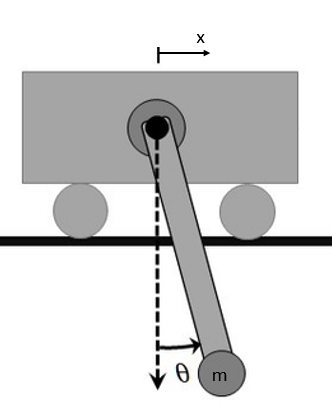
\includegraphics[width=.8\linewidth]{pendulumoncart.png}
		\captionof{figure}{Depiction of the pendulum placed on the cart \cite{Quanser} }
		\label{fig:pendulumoncart}
	\end{minipage}%
	\begin{minipage}{.5\textwidth}
		\centering
		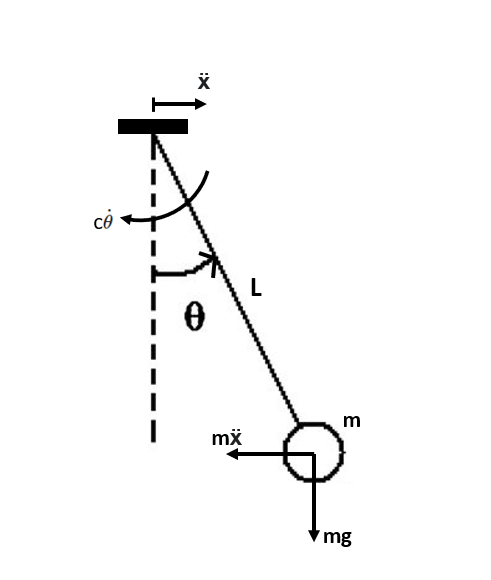
\includegraphics[width=0.8\linewidth]{VLDpendulum.png}
		\captionof{figure}{Free body diagram of the pendulum \cite{Researchgate}}
		\label{fig:VLDpendulum}
	\end{minipage}
\end{figure*}


\subsection{State-space Equation for the non-linear Model}
To derive a state-space equation for the non-linear model, following states are used:
\begin{equation}
	\xi = [x, \theta, L\dot{\theta} +  \dot{x}\cos(\theta)]^{T}
\end{equation}
In this state vector, $x$ stands for the position of the cart and $\theta$ stands for the pendulum angle. In the third state $L\dot{\theta} +  \dot{x}\cos(\theta)$, the tangential velocity of the centre of gravity of the pendulum with relation to a standstill reference frame can be recognized. For this reason, we will call the third state $v_{tan}$ from now on. The state vector then becomes: 
\begin{equation}
\xi = [x, \theta, v_{tan}]^{T}
\label{eq:xi}
\end{equation}
Using Equation \ref{eq:newton} and the definition of $\xi$, the nonlinear state-space equation can be derived. The input is the velocity of the cart and is denoted as $v_{c}$. 

\begin{equation}
	\dot{\xi} = \mathbf{f}(\xi,v_c) = \begin{bmatrix}
	\dot{x} \\ \dot{\theta} \\ L\ddot{\theta} + \ddot{x}\cos(\theta) - \dot{x}\sin(\theta)\dot{\theta}
	\end{bmatrix} = \begin{bmatrix}
	v_c \\ \frac{v_{tan}-v_c\cos(\theta)}{L} \\ -g\sin(\theta) - (\frac{c}{mL}+v_c\sin(\theta))(\frac{v_{tan} - v_c\cos(\theta)}{L})
	\end{bmatrix}
	\label{eq:nonlinear}
	\end{equation}
	\begin{equation}
	\mathbf{y} 
 = \begin{bmatrix}
	 x\\\theta
 \end{bmatrix} = \begin{bmatrix}
 1&0&0\\0&1&0
 \end{bmatrix}\xi + 0 \cdot v_c
 \label{eq:measurementnonlinear}
 \end{equation}




\subsection{Linearization of the Model}
\label{sec:linearization}
The nonlinear model can be linearized around the equilibrium state $\mathbf{\xi_0}$ = $[0,0,0]^T$. Both $\theta$ and $v_{tan}$ have to be zero in the equilibrium state. The value of $x$ doesn't really matter, but is taken equal to zero for convenience. The equilibrium input $v_{c0}$ is also chosen to be equal to zero. Calculating the jacobian matrices \textbf{F} and \textbf{G}, we can rewrite the model as:
\begin{equation}
	\delta\mathbf{\dot{\xi}} = \mathbf{F}\delta\mathbf{\xi} + \mathbf{G}\delta v_c
	\label{eq:deltaxidotlinear}
	\end{equation}
	Where $\delta\mathbf{\xi}$ and $\delta v_c$ are defined as follows:
	\begin{equation}
	\begin{split}
	\delta\mathbf{\xi} &= \xi - \xi_0 = \xi \\
	\delta v_c &= v_c - v_{c0} = v_c
	\end{split}
	\end{equation}
	Using nonlinear Equation \ref{eq:nonlinear}, $\mathbf{F}$ and $\mathbf{G}$ are defined as: 
	\begin{equation}
	\begin{split}
	\mathbf{F} &= \frac{\partial \mathbf{f}}{\partial \xi}\Bigr|_{\xi_0, v_{c0}}\\
	\mathbf{G} &= \frac{\partial \mathbf{f}}{\partial v_{c}}\Bigr|_{\xi_0, v_{c0}}
	\end{split}	
	\label{eq:jacobians}
	\end{equation}
	From Equation \ref{eq:jacobians}, the following matrices arise:
	\begin{equation}
	\begin{split}
	\mathbf{F} &= \begin{bmatrix}
	0&0&0\\0&0&\frac{1}{L}\\0&-g&\frac{-c}{mL^2}
	\end{bmatrix}\\
	\mathbf{G} &= \begin{bmatrix}
	1\\\frac{-1}{L}\\\frac{c}{mL^2}
	\end{bmatrix}
	\end{split}
	\end{equation}
	As the measurement equation was already linear, we find the following linear state-space model:
	
	\begin{equation}
	\label{eq:sslinear}
	\delta\mathbf{\dot{\xi}} = \begin{bmatrix}
	0&0&0\\0&0&\frac{1}{L}\\0&-g&\frac{-c}{mL^2}
	\end{bmatrix} \delta\xi + \begin{bmatrix}
	1\\\frac{-1}{L}\\\frac{c}{mL^2}
	\end{bmatrix} \delta v_c
	\end{equation}
	\begin{equation}
	\mathbf{y} 
	= \begin{bmatrix}
	x\\\theta
	\end{bmatrix} = \begin{bmatrix}
	1&0&0\\0&1&0
	\end{bmatrix}\xi + 0 \cdot v_c
	\label{eq:measurementlinear}
\end{equation}
By applying the laplace transformation to Equation \ref{eq:sslinear}, following transfer functions can be found. 

\begin{equation}
\begin{split}
\frac{d\delta x}{dt} = v_c &\rightarrow H_x(s) = \frac{\delta X(s)}{\delta V_c(s)} = \frac{1}{s}\\
\frac{d\delta \theta}{dt} = \frac{v_{tan}-v_c}{L} &\rightarrow H_{\theta}(s) = \frac{\delta \Theta(s)}{\delta V_c(s)} = \frac{-1}{sL}\\
\frac{d\delta v_{tan}}{dt} = -g\delta\theta - \frac{c}{mL^2}\delta v_{tan} +  \frac{c}{mL^2} \delta v_c &\rightarrow H_{v_{tan}}(s) = \frac{\delta V_{tan}(s)}{\delta V_c(s)} = \frac{1}{\frac{mL^2}{c}s+1}
\end{split}
\end{equation}


\subsection{Determination of the Pendulum Length}
The damping ratio $\zeta$ can be determined, using the logarithmic decrement. In this experiment, the maximal amplitude of the angle $\theta$ for two consecutive periods are measured. This is shown in Figure \ref{fig:logdecrement}, where T stands for the period of the oscillation. The logarithmic decrement $\delta$ is then defined as \cite{slidestrillingen}:
\begin{equation}
	\delta = ln\bigg(\frac{\theta(t)}{\theta(t+T)}\bigg) = \frac{2\pi\zeta}{\sqrt{1-\zeta^2}}
	\label{eq:delta}
	\end{equation}
	Where $\theta(t)$ and $\theta(t+T)$ are both the values of the maximal angle in their period. From Equation \ref{eq:delta}, $\zeta$ can be derived:
	\begin{equation}
	\zeta = \frac{\delta}{\sqrt{(2\pi)^2+\delta^2}}
\end{equation}
By measuring the period of the oscillations, the distance $L$ from the rotating point to the centre of gravity can be calculated. since the pendulum has two bolts detached at the end of it, the centre of gravity will be located close to the end, but the distributed mass of the pendulum will cause the calculated length $L$ to be smaller than the measured length from the rotating point to the end of the pendulum $L_m$.
\\\\\
From the measured period, we can derive the measured (damped) pulsation, which is an estimate for the real pulsation. 
\begin{equation}
	\omega_d = \frac{2\pi}{T} = \omega_n\sqrt{1-\zeta^2}
	\label{eq:wd}
	\end{equation}
	From Equation \ref{eq:wd}, the natural pulastion $\omega_n$ can be derived. As $\omega_n = \sqrt{\frac{g}{L}}$, L can be found as:
	\begin{equation}
	L = \frac{g}{\omega_n^2} = \frac{g(1-\zeta^2)}{\omega_d^2}
\end{equation}


\begin{figure}[htp!]
	\centering
	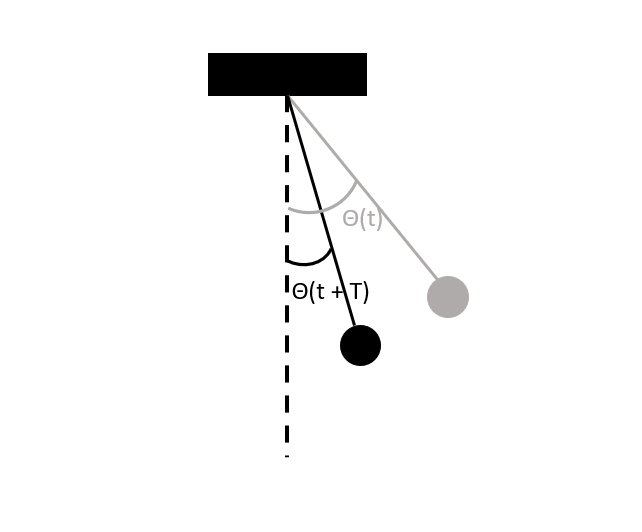
\includegraphics[width=0.5\linewidth]{logdecrement.png}
	\caption{Measured values for the experiment to determine $\zeta$}
	\label{fig:logdecrement}
\end{figure}
\noindent The numerical values are: $T = 0.71s$, $L = 0.1258m$, $\zeta = 0.0327 [-]$. As expected, the measured length $L_m = 0.151m$ is larger than de calculated length $L$. If the damping is neglected, the measured pulsation $\omega_d$ is equal to the natural pulsation $\omega_n$ and the length can be calculated as $L' = \frac{g}{\omega_d^2} = 0.1259m$.
\\\\
The damping coefficient $c$ is related to the damping ratio $\zeta$ via Equation \ref{eq:c}. As the pendulum mass is unknown, the moment of inertia $J$ is unknown and $c$ can not be calculated. 

\begin{equation}
		\zeta = \frac{c}{c_{crit}} = \frac{c}{2J\omega_n}
		\label{eq:c}
\end{equation}

\noindent\textbf{Important note:} For the remainder of this report, the damping will be neglected.
\subsection{Discretization}
\subsubsection*{Linear model}
To discretize the linear model, the forward Euler method is used:
\begin{equation}
	\delta\dot{\xi} = \frac{\delta\xi[k+1]-\delta\xi[k]}{T_s}
	\label{eq:FElinear}
\end{equation}
Filling in Equation \ref{eq:FElinear} in Equation \ref{eq:deltaxidotlinear} yields the following equation:
\begin{equation}
	\delta\xi[k+1] = (\mathbf{I} + T_s\mathbf{F})\delta\xi[k] + T_s\mathbf{G}\delta v_c[k]
	\end{equation}
	Which can be translated into the following discretized, linear state-space model (where the damping is neglected, $c = 0$):
	\begin{equation}
	\begin{split}
	\delta\xi[k+1] &= \begin{bmatrix}
	1&0&0\\0&1&\frac{T_s}{L}\\0&-gT_s&1
	\end{bmatrix}\delta\xi[k] + \begin{bmatrix}
	T_s\\ \frac{-T_s}{L}\\0
	\end{bmatrix}v_c[k]\\
	\begin{bmatrix}
	x[k]\\\theta[k]
	\end{bmatrix} &= \begin{bmatrix}
	1&0&0\\0&1&0
	\end{bmatrix}\xi[k] + 0 \cdot v_c[k]
	\end{split}
\end{equation}
\subsubsection*{Non-linear model}
To discretize the non-linear model, the forward Euler method is used as well:
\begin{equation}
	\dot{\xi} = \frac{\xi[k+1]-\xi[k]}{T_s}
	\label{eq:FEnonlinear}
	\end{equation}
	By filling in Equation \ref{eq:FEnonlinear} in Equation \ref{eq:nonlinear} the following equation can be derived:
	\begin{equation}
	\xi[k+1] = T_s\mathbf{f}(\xi[k],v_c[k]) + \xi[k]
	\end{equation}
	By neglecting the damping of the system, following discretized, nonlinear state-space model can be found:
	\begin{equation}
	\xi[k+1] = \begin{bmatrix}
	T_sv_c[k] + x[k]\\T_s\cdot\frac{v_{tan}[k] - v_c[k]\cos(\theta[k])}{L} + \theta[k]\\
	T_s\bigg(-g\sin(\theta[k]) - v_c[k]\sin(\theta[k])\frac{v_{tan}[k]-v_c[k]\cos(\theta[k])}{L}\bigg) + v_{tan}[k]
	\end{bmatrix}
	\label{eq:ssnonlineardiscrete}
	\end{equation}
	\begin{equation}
	\begin{bmatrix}
	x[k]\\\theta[k]
	\end{bmatrix} = \begin{bmatrix}
	1&0&0\\0&1&0
	\end{bmatrix}\xi[k] + 0 \cdot v_c[k]
	\label{eq:measurementlineardiscrete}
	\end{equation}
	
	\section{Design and implementation of a linear Kalman filter}
	The linearized measurement equation is given by Equation \ref{eq:measurementlineardiscrete}.
	\underline{GRAFIEKEN + UITLEG}
	
	\section{Design and implementation of an extended Kalman filter}
	\subsection{Nonlinear measurement equation}
	As is already written down in the nonlinear state-space model Equations \ref{eq:measurementnonlinear}, the measurement equation based on the nonlinear system equations is actually a linear equation. This is caused by the fact that the two outputs $x$ and $\theta$ are two states. The measurement equation based on the nonlinear system equations can be written as:
	\begin{equation}
	\mathbf{y} = \begin{bmatrix}
	x\\\theta
	\end{bmatrix} = \mathbf{g}(\xi,v_c) = \begin{bmatrix}
	1&0&0\\0&1&0
	\end{bmatrix}\xi + 0 \cdot v_c
	\label{eq:g}
\end{equation}
\subsection{Jacobian of the state and measurement equation}
The Jacobian matrix of the state equation and the Jacobian matrix of the measurement equation can be found by taking the derivative of the functions \textbf{f} (Equation \ref{eq:ssnonlineardiscrete}) and \textbf{g} (Equation \ref{eq:g}) to the state vector $\xi$

\begin{equation}
\begin{split}
\mathbf{A} &= \frac{\partial \mathbf{f}}{\partial \xi}\\
\mathbf{C} &= \frac{\partial \mathbf{g}}{\partial \xi}
\end{split}	
\label{eq:jacobiannotequilibrium}
\end{equation}
Unlike the linear Kalman filter, the extended Kalman filter uses discretized jacobian matrices evaluated in the current state estimate and not in the equilibrium state. Using Equations \ref{eq:jacobiannotequilibrium}, following expressions can be derived for the discrete time jacobians, starting from nonlinear, discrete state-space model \ref{eq:ssnonlineardiscrete}. Damping is neglected: 
\begin{equation}
\begin{split}
\mathbf{A} &= \begin{bmatrix}
1&0&0\\0&1+T_s\frac{v_c\sin(\theta)}{L}&\frac{T_s}{L}\\0&T_s\bigg(-g\cos(\theta) - \frac{v_{tan}-v_c\cos(\theta)}{L} \cdot v_c \cos(\theta)-\frac{(v_c\sin(\theta))^2}{L}\bigg)&1+T_s\frac{-v_c\sin(\theta)}{L}
\end{bmatrix}\\
\mathbf{C} &= \begin{bmatrix}
1&0&0\\0&1&0
\end{bmatrix}
\end{split}
\end{equation}
\subsection{Implementation of the extended Kalman filter}
Since the linearization of the model has no influence on the measurement noise covariance or the covariance of the initial state estimation errors, the values for $\mathbf{R}$ and $\mathbf{\hat{P}}_{0|0}$ for the extended Kalman filter are taken equal to those used in the linear Kalman filter (see Equations \underline{VERWIJZEN NAAR VROEGERE MATRICES}). As the nonlinear model is used for the extended Kalman filter, the model should be more precise and thus the proces noise should be lower. For this reason $\mathbf{Q}$ is taken one order of magnitude smaller than the $\mathbf{Q}$ used in the linear Kalman filter. 
\begin{equation}
	\mathbf{Q} = \begin{bmatrix}
	2.7878\cdot10^{-9}&0&0\\0&2.3511\cdot10^{-9}&0\\0&0&10^{-5}
	\end{bmatrix}
	\end{equation}
	\underline{GRAFIEKEN + UITLEG}
	
	\section{Design and implementation of a state feedback controller based on the linearized model}
	\subsection{Design of a linear quadratic regulator}
	The objective of the LQR is to find the control input $v_c[k]$ that moves the system states $\xi \neq 0$ to \textbf{0}, in a way the performance criterion $\J$ is minimized. This means a tradeoff has to be made between performane $\J_p$, the speed with which the states go to zero (or a desired state), and the controll effort $\J_c$. The criterion is given in Equation \ref{eq:criterionLQR}. 
	\begin{equation}
	\J = \J_p + \J_c =  \sum_{k=0}^{\infty}\mathbf{\xi}[k]^T\mathbf{Q}\mathbf{\xi}[k] + v_c[k]Rv_c[k]
	\label{eq:criterionLQR}
	\end{equation}
	The matrix \textbf{Q} and the value R are design parameters. These values determine which part of the tradeoff is most important in this particular design: performance or control effort. The tuning of the parameters and thus the design of the LQR itself is done in Section \ref{sec:implFBcontr}. 
	
	\subsection{Design of a feedforward gain}
	
	The blockdiagram of the system with feedforward compensation can be found in Figure \ref{fig:blockdiagram}. 
	
	\begin{figure*}[htp!]
		\centering
		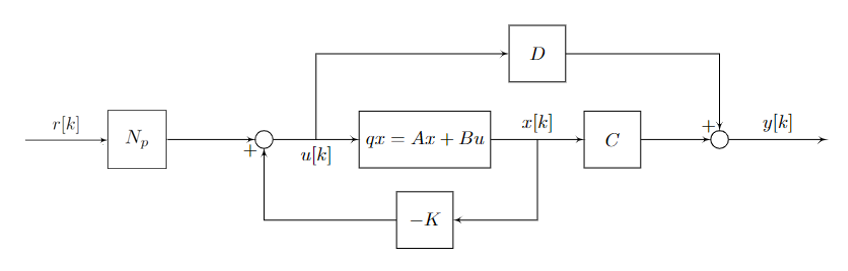
\includegraphics[width=.7\linewidth]{blockdiagram.png}
		\caption{Blockdiagram of the system with feedforward compensation }
		\label{fig:blockdiagram}
	\end{figure*}
	The feedforward gain $N_p$ is calculated such that the steady-state error equals zero for a step reference in desired position, which is denoted with $r[k]$. The pendulum mass position can be written as:
	\begin{equation}
	x_p = x + L\cdot \sin(\theta) = x + L\cdot \theta
	\end{equation}
	$x_p$ is thus a linear combination of the two outputs of the linear system. The total transfer function \textbf{H}(z) of the system is thus a vector containing 2 transfer functions: $H_x(z) = \frac{X(z)}{V_c(z)}$ and $\frac{\Theta(z)}{V_c(z)}$. The pendulum mass position can be calculated starting from a given $v_c$ as follows:
	\begin{equation}
	X_p(z) = (H_x(z) + LH_\theta(z))V_c(z)
	\end{equation}
	Following the reasoning on C9, slide 54 of the slides of the course Control Theory \cite{slidescontroltheory}, the expression for $N_p$ to 
	
	\subsection{Implementation of the controller}
	\label{sec:implFBcontr}
	
	\bibliographystyle{plain}
	\bibliography{bibliography}
	
\end{document}